\documentclass[a4paper,11pt,english]{article}
\usepackage{standalone}
\usepackage{tikz}
\usetikzlibrary{decorations.pathreplacing,arrows.meta,shapes}
\usepackage{tcolorbox}
\tcbuselibrary{breakable,skins}
\usepackage{algorithm}
\usepackage{algpseudocode}
\usepackage{babel}
\usepackage{booktabs}
\usepackage[colorlinks,pdfstartview=FitH,bookmarks,pdfcenterwindow]{hyperref}
\usepackage[capitalise]{cleveref}

\usepackage{protocol_version}

\definecolor{base03}{RGB}{000, 043, 054}
\definecolor{base02}{RGB}{007, 054, 066}
\definecolor{base01}{RGB}{088, 110, 117}
\definecolor{base00}{RGB}{101, 123, 131}
\definecolor{base0}{RGB}{131, 148, 150}
\definecolor{base1}{RGB}{147, 161, 161}
\definecolor{base2}{RGB}{238, 232, 213}
\definecolor{base3}{RGB}{253, 246, 227}
\definecolor{yellow}{RGB}{181, 137, 000}
\definecolor{orange}{RGB}{203, 075, 022}
\definecolor{red}{RGB}{220, 050, 047}
\definecolor{magenta}{RGB}{211, 054, 130}
\definecolor{violet}{RGB}{108, 113, 196}
\definecolor{blue}{RGB}{038, 139, 210}
\definecolor{cyan}{RGB}{042, 161, 152}
\definecolor{green}{RGB}{133, 153, 000}

\makeatletter

\def\@autolabel#1{%
\expandafter\let\csname old#1\expandafter\endcsname\csname#1\endcsname
\expandafter\def\csname @#1@label\endcsname[##1]##2{\csname old#1\endcsname{##2}\label{s:##1}}
\expandafter\def\csname #1\endcsname{\expandafter\@ifnextchar[{\csname @#1@label\endcsname}{\csname old#1\endcsname}}
}

\@autolabel{part}
\@autolabel{section}
\@autolabel{subsection}
\@autolabel{subsubsection}
\@autolabel{paragraph}
\@autolabel{subparagraph}

\makeatother

\newtcolorbox{admobox}[3][]{
  breakable, skin=enhancedmiddle,
  boxrule=0mm, leftrule=2mm,
  colframe=#3, colback=#3!10, coltext=#3!30!black,
  title={#2}, attach title to upper, after title={.\ },
  fonttitle={\bfseries}, coltitle=black,
  #1
}
\def\notebox#1#2{
  \begin{admobox}{#1}{blue}
  #2
  \end{admobox}
}
\def\warnbox#1#2{
  \begin{admobox}{#1}{yellow}
  #2
  \end{admobox}
}
\def\errorbox#1#2{
  \begin{admobox}{#1}{red}
  #2
  \end{admobox}
}
\def\tipbox#1#2{
  \begin{admobox}{#1}{green}
  #2
  \end{admobox}
}

\def\fieldsize#1{
  \tikz[baseline=-.5ex]{
    \tikzset{fieldsize/.style={
      rectangle split,
      rectangle split parts=2,
      rectangle split horizontal,
      rectangle split part fill={violet,violet!10},
      rectangle split draw splits=false,
      rounded corners=2pt,
      rectangle split part align=base,
      draw=violet,
    }}
    \node[fieldsize] (var) {\textsc{\color{white}Size}\nodepart[text=violet!50!black]{two}#1};
  }
}

\floatname{algorithm}{Listing}
\renewcommand{\listalgorithmname}{List of Listings}
\crefname{algorithm}{Listing}{Listings}

\algnewcommand\texttype{\textsc}
\algnewcommand\algorithmicstruct{\textbf{struct}}
\algdef{SE}[STRUCT]{Struct}{EndStruct}[1]{\algorithmicstruct\ \texttype{#1}}{\algorithmicend\ \algorithmicstruct}
\def\t#1:#2;{\ensuremath{#1}\ :\ #2}
\def\T{\State\t}
\def\acc{\ensuremath{\rightarrow}}

\title{OrbiPacket Protocol Specification - v\version}
\author{The OrbiSat Oeiras Team}
\date{}

\begin{document}
\maketitle
\documentclass{standalone}
\usepackage{tikz}
\usetikzlibrary{decorations.pathreplacing,arrows.meta}


\begin{document}
\definecolor{base03}{RGB}{000, 043, 054}%
\definecolor{base02}{RGB}{007, 054, 066}%
\definecolor{base01}{RGB}{088, 110, 117}%
\definecolor{base00}{RGB}{101, 123, 131}%
\definecolor{base0}{RGB}{131, 148, 150}%
\definecolor{base1}{RGB}{147, 161, 161}%
\definecolor{base2}{RGB}{238, 232, 213}%
\definecolor{base3}{RGB}{253, 246, 227}%
\definecolor{yellow}{RGB}{181, 137, 000}%
\definecolor{orange}{RGB}{203, 075, 022}%
\definecolor{red}{RGB}{220, 050, 047}%
\definecolor{magenta}{RGB}{211, 054, 130}%
\definecolor{violet}{RGB}{108, 113, 196}%
\definecolor{blue}{RGB}{038, 139, 210}%
\definecolor{cyan}{RGB}{042, 161, 152}%
\definecolor{green}{RGB}{133, 153, 000}%
\def\field[#1](#2)(#3)#4{\fill[#1,draw=base03] (#2) rectangle ++(#3) node[midway,text=base3,align=center] {#4};}%
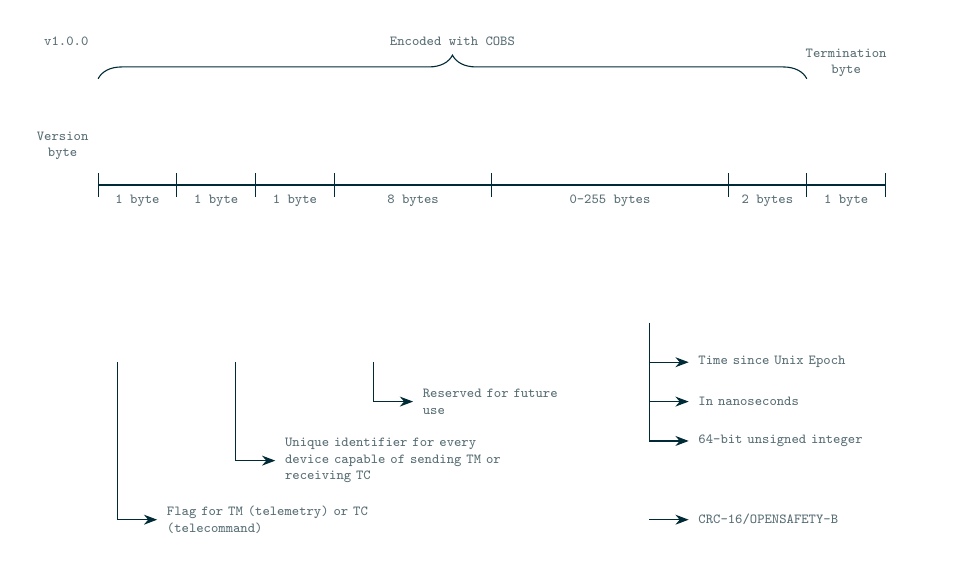
\begin{tikzpicture}[yscale=-1,draw=base03,every node/.style={font=\tiny\ttfamily,text=base01}]
\node[above left] at (0,-.4) {v1.0.0};
% Full packet
\field[blue](0,0)(5,.5){HEADER}
\field[base02](0,.5)(1,.5){0x01}
\field[violet](1,.5)(1,.5){LENGTH}
\field[magenta](2,.5)(1,.5){CONTROL}
\field[cyan](3,.5)(2,.5){TIMESTAMP}
\field[base00](5,0)(3,1){PAYLOAD}
\field[green](8,0)(1,1){CRC}
\field[base02](9,0)(1,1){0x00}
% Field sizes
\draw (0,1.25) -- ++(10,0);
\foreach\x in {0,1,2,3,5,8,9,10}{
\draw (\x,1.1) -- ++(0,.3);
}
\node[below] at (.5,1.25) {1 byte};
\node[below] at (1.5,1.25) {1 byte};
\node[below] at (2.5,1.25) {1 byte};
\node[below] at (4,1.25) {8 bytes};
\node[below] at (6.5,1.25) {0-255 bytes};
\node[below] at (8.5,1.25) {2 bytes};
\node[below] at (9.5,1.25) {1 byte};
% Annotations
\node[left,align=center] at (0,.75) {Version\\byte};
\node[above,align=center] at (9.5,0) {Termination\\byte};
\draw[decorate,decoration={brace,amplitude=.3cm}] (0,-.1) -- ++(9,0) node [midway,above=.3cm] {Encoded with COBS};
% Control byte
\field[magenta](0,2.5)(4,.5){CONTROL}
\field[yellow](0,3)(.5,.5){TM/\\TC}
\field[orange](.5,3)(2.5,.5){DEVICE ID}
\field[red](3,3)(1,.5){RESERVED}
\draw[-Stealth] (3.5,3.5) |- ++(.5,.5) node[right,align=left,text width=2cm] {Reserved for future use};
\draw[-Stealth] (1.75,3.5) |- ++(.5,1.25) node[right,align=left,text width=3cm] {Unique identifier for every device capable of sending TM or receiving TC};
\draw[-Stealth] (.25,3.5) |- ++(.5,2) node[right,align=left,text width=3cm] {Flag for TM (telemetry) or TC (telecommand)};
% Timestamp
\field[cyan](6,2.5)(2,.5){TIMESTAMP}
\draw[-Stealth] (7,3) |- ++(.5,.5) node[right,align=left,text width=3cm] {Time since Unix Epoch};
\draw[-Stealth] (7,3) |- ++(.5,1) node[right,align=left,text width=3cm] {In nanoseconds};
\draw[-Stealth] (7,3) |- ++(.5,1.5) node[right,align=left,text width=3cm] {64-bit unsigned integer};
% Crc
\field[green](6,5)(1,1){CRC}
\draw[-Stealth] (7,5.5) -- ++(.5,0) node[right,align=left]{CRC-16/OPENSAFETY-B};
\end{tikzpicture}
\end{document}
\tableofcontents

\section[intro]{Introduction}

OrbiPacket is a packet-based communication protocol. It was created specifically for communication with CanSat\footnotemark\ devices. These devices can be fitted with very diverse electronics, and are often resource-constrained. Thus, this protocol has the goals of being simple and easy to use while providing decent efficiency and minimal overhead.

\footnotetext{CanSat's are small electronic devices, sized and shaped similarly to a soda can. They are used to perform various kinds of scientific missions, usually being released by rockets or other devices at varying altitudes. The \textit{European Space Education Resource Office} (ESERO) holds CanSat competitions in various member states, challenging teams of secondary education students to build their own CanSat.}

\notebox{A bit of history}{
  The OrbiSat Oeiras team first participated in the CanSat Portugal competition in 2023/2024, being one of the finalists of the 11th edition. Several issues on all fronts meant no data was received during the CanSat's descent. The next year, wanting to get everything right, the team's firmware developer (aka me, Levi Gomes) decided sending data over text was neither efficient nor rigorous enough. So, after some effort, the first version of OrbiPacket was born during the 12th edition of the competition, in 2024/2025. And in case you're curious... no, we still didn't get any data.
}

\section[overview]{Protocol Overview}
The OrbiPacket protocol enables communication between a CanSat and one or more groundstations. This communication is carried out by exchanging \textbf{packets}, the basic units of the protocol. Packets are autonomous entities, which have a logical, high-level structure. These packets can be converted into raw bytes -- a process known as \textbf{encoding} -- adequate for transmission over a physical layer\footnotemark (e.g. radio). At the other end of the link, the received bytes can then be \textbf{decoded} back into packets.

\footnotetext{In this specification, the designation \textit{physical layer} is used very liberally, referring to any layers responsible for transmitting raw bytes. In that sense, the physical layer refers to the set of all layers below OrbiPacket -- which might be a single layer or multiple layers.}

For communication to be possible, messages aren't enough -- one also requires \textit{communicators}. In OrbiPacket, these communicators are referred to as \textbf{devices}. A device is any discrete entity capable of sending and receiving packets. Note that OrbiPacket devices don't need to correspond to physical devices. In fact, a single piece of hardware can act as several devices, or, conversely, many components can come together under one device.

The protocol distinguishes between two kinds of packets: \textbf{telemetry} (TM) and \textbf{telecommand} (TC). The former represent data being sent \textit{from} a device, whereas the latter encodes instructions sent \textit{to} a device.

As an example, consider a temperature sensor which is able to send readings and receive a command to alter the frequency of said readings. The readings will be wrapped in TM packets, while the command will be a TC packet. Since the sensor is able to send and receive packets, it is considered a device.

It is important to note that devices are more than a formalism. Each packet contains information about the device it relates to (i.e. the sender for TM packets and the receiver for TC packets), in the form of a \textbf{device identifier} (ID). The ID is a 5-bit number uniquely identifying a device in the CanSat.

\section[fields]{Packet Structure}

A packet is made up of several \textit{fields}. \Cref{table:struct} shows an overview of the packet structure. The fields before the payload are called the \textbf{header}, they contain metadata about the packet. When encoding a packet, fields must be concatenated in order. Fields which span multiple bytes are to be encoded in \textbf{little endian}, i.e., least-significant byte first.

\begin{table}[h]
  \centering
  \begin{tabular}{lr}
    \toprule
    Field            & Size (bytes) \\
    \midrule
    Version          & 1            \\
    Length           & 1            \\
    Control          & 1            \\
    Timestamp        & 8            \\
    Payload          & 0-255        \\
    CRC              & 2            \\
    Termination Byte & 1            \\
    \bottomrule
  \end{tabular}
  \caption{Packet structure overview}
  \label{table:struct}
\end{table}

\subsection[f:header]{Header}

\subsubsection[f:version]{Version}
\fieldsize{1 byte}\\[8pt]
Indicates the protocol version. Breaking updates to the protocol increment this field to ensure backwards compatibility. The current version of the protocol (\version) specifies \texttt{0x\versionbyte} as the version byte.


\subsubsection[f:length]{Length}
\fieldsize{1 byte}\\[8pt]
Specifies the size of the payload in bytes, ranging from 0 to 255.


\subsubsection[f:control]{Control}
\fieldsize{1 byte}\\[8pt]
Encodes metadata about the packet kind and device identifier. The following fields are specified from the highest bit to the lowest bit.
\begin{itemize}
  \item \textbf{TM/TC Flag}: 1 bit, where \texttt{0} indicates telemetry and \texttt{1} indicates a telecommand.
  \item \textbf{Device ID}: 5 bits, uniquely identifying the source device for TM or target device for TC. Note that device IDs should remain consistent across TM and TC packets.
\end{itemize}
\warnbox{Reserved bits}{
  The two remaining bits of the control byte are currently unused. Future versions of the protocol may use them to include additional information. They must therefore be ignored -- do not use them to encode application specific data.
}
\tipbox{Interpreting the control byte}{
  One can think of the control byte as \textit{saying} the following about the packet:
  \begin{itemize}
    \item \texttt{0b0DDDDDRR}: TM packet from device \texttt{0bDDDDD} to the groundstation
    \item \texttt{0b1DDDDDRR}: TC packet from the groundstation to device \texttt{0bDDDDD}
  \end{itemize}
}


\subsubsection[f:timestamp]{Timestamp}
\fieldsize{8 bytes}\\[8pt]
Represents the time since the Unix epoch in nanoseconds as a 64-bit unsigned integer.


\subsection[f:payload]{Payload}
\fieldsize{0–255 bytes}\\[8pt]
Contains application-specific data, such as telemetry readings or command instructions. The structure of the payload is currently up to the application, but that may be subject to change in future versions.


\subsection[f:crc]{CRC}
\fieldsize{2 bytes}\\[8pt]
Cyclic redundancy check value computed over all preceding fields. The generator polynomial used by the protocol is \href{https://reveng.sourceforge.io/crc-catalogue/all.htm#crc.cat.crc-16-opensafety-b}{CRC-16/OPENSAFETY-B}, or \texttt{0xbaad} in Koopman's notation.


\subsection[f:term]{Termination Byte}
\fieldsize{1 byte}\\[8pt]
Inserted at the end of every packet to frame it, i.e, delimit it from adjacent packets. Fixed at \texttt{0x00}.

\subsection[repr]{Representation}
In their unencoded form, packets should be represented by a high-level construct. The specifics of this will invariably depend on the concrete language. Nonetheless, the recommended way of representing packets is through the use of a custom data type or object.

In the following sections, the pseudo-code data type defined in \cref{listing:struct} will be used. Notice the CRC field isn't included in the representation, since it is not part of the packet's information, and should only exist in the encoded form. For simplicity, the length field isn't included, under the assumption that is can be retrieved from the array holding the payload. If such is not possible or practical due to language-specific constraints, it must be included in the packet representation.

\begin{algorithm}[h]
  \caption{Packet Representation}\label{listing:struct}
  \begin{algorithmic}[1]
    \Struct{Packet}
    \T version:uint8;
    \T kind:TM or TC;
    \T deviceId:uint8;
    \T timestamp:uint64;
    \T payload:uint8[];
    \EndStruct
  \end{algorithmic}
\end{algorithm}

\subsection[payload-enc]{Payload Storage}
A payload can contain arbitrary data -- as long as it doesn't surpass the 255 byte limit. This data could assume many forms, and thus be of many different data types, which all have to somehow be stored by the same representation.

Perhaps the most obvious solution for many would be the use of a generic type (or a type template, or whichever other name such a construct might have). Thus the representation presented in \cref{listing:struct} would become something like \cref{listing:struct-generic}. While it might seem good at first, this solution presents two major drawbacks. Firstly, there are languages that don't support generics. Out of those that do, not all provide a mechanism to restrict the generic argument based on its size, so payloads over 255 bytes would only be detected when attempting to encode them. Furthermore, generics tend to \textit{pollute} APIs -- if packets were generic, any function or type interacting with them would also have to be generic. Because of these downsides, this solution is deemed unfitting.

\begin{algorithm}[h]
  \caption{A generic packet}\label{listing:struct-generic}
  \begin{algorithmic}[1]
    \Struct{Packet<P>}
    \T version:uint8;
    \T kind:TM or TC;
    \T deviceId:uint8;
    \T timestamp:uint64;
    \T payload:P;
    \EndStruct
  \end{algorithmic}
\end{algorithm}

Another possibility would be to use a \textit{universal} type\footnotemark\ which can hold anything. Once again, this approach has the issue of not being able to reject payloads larger than 255 bytes when they're created. On top of that, universal types are usually unsafe to handle, since all type information is lost.

\footnotetext{This is known by many names. In type theory, it's often referred to as \textit{top} or \textit{any}; object oriented languages usually call it \textit{object}.}

The third option, and the one currently chosen by OrbiPacket, is to store the raw bytes of the payload in the packet representation, as a byte array. This way, any form of data can be stored -- and by using fixed-size arrays, a payload larger than 255 bytes can't ever be created. In effect, this solution offsets the conversion of a payload to its bytes from the time of packet encoding to the time of packet creation. However, this doesn't mean the end-user should be responsible for performing the conversion -- that would be potentially unsafe.\footnotemark\ Instead, an implementation should provide an API to create payloads out of common data types.

\footnotetext{For instance, an end-user could mistakenly provide the bytes in big-endian.}

\section[enc]{Encoding}

Encoding a packet is the process of converting it into a stream of bytes. This stream of bytes is written into a buffer (byte array), either provided by the end-user or managed by the implementation.

Firstly, the packet's header fields are written to the buffer in order. The control byte is constructed from the packet kind and the device ID, using appropriate bitwise operations. The timestamp is written in little-endian, i.e., least-significant byte first. As previously discussed, payloads are stored as a byte array, which is simply copied to the buffer. Then, a CRC is computed over the buffer. The resulting 2 bytes are appended to the buffer, in little-endian. The buffer is then stuffed -- see \cref{s:stuff}, and finally a termination byte is appended.

\subsection[stuff]{Stuffing}

To prevent the occurrence of the termination byte (\texttt{0x00}) within the packet, which would lead to framing errors, the protocol employs \textbf{COBS (Consistent Overhead Byte Stuffing)}. This stuffing is applied to all fields except the termination byte itself.

A full explanation of COBS is beyond the scope of this specification -- if necessary, refer to the literature on the subject. In short, COBS works by replacing every null byte with the \textit{distance} to the next null byte -- this also includes prepending a byte indicating the distance to the first null byte. Furthermore, if the distance to the next null byte is larger than 255 (the maximum value of a single byte), then a distance of 255 will be indicated, and the 255$^{th}$ byte will then indicate the distance to the next null byte (which can again be 255). Not only is this process remarkably simple, it also guarantees \textit{consistent overhead}, i.e., the best-case, average-case and worst-case overheads are quite similar. The worst-case overhead is
$$\left\lceil \frac{N}{254} \right\rceil\,,$$
where $N$ is the length of the input.

\subsection[enc-impl]{Implementation details}
\Cref{listing:enc-pseudo} presents an encoding procedure in pseudo-code, to serve as a reference for implementations. The procedure should be part of the public API of the implementation, taking in an instance of a packet (according to the representation presented in \cref{s:repr}), and possibly a buffer. It should return a buffer (or a view into one) containing the encoded packet, possibly wrapped in a result type if any operations it performs are fallible. For implementations in object-oriented languages, it is recommended this method is a member of the representation object type.

\begin{algorithm}[h]
  \caption{Encoding Procedure}\label{listing:enc-pseudo}
  \begin{algorithmic}
    \Procedure{encode}{\t packet:Packet;}
    \State $\textit{buffer} \gets []$
    \State write $\textit{packet} \acc \textit{version}$ to \textit{buffer}
    \State write (length of $\textit{packet} \acc \textit{payload}$) to \textit{buffer}
    \State $\textit{control} \gets \left(\textit{packet} \acc \textit{deviceId} \ll 2\right)$
    \If{$\textit{packet} \acc \textit{kind}$ is TC}
    \State $\textit{control} \gets \textit{control} \mathbin{|} \texttt{0b10000000}$
    \EndIf
    \State write \textit{control} to \textit{buffer}
    \State write (little-endian bytes of $\textit{packet} \acc \textit{timestamp}$) to \textit{buffer}
    \State write $\textit{packet} \acc \textit{payload}$ to \textit{buffer}
    \State write (compute CRC of \textit{buffer}) to \textit{buffer}
    \State stuff \textit{buffer}
    \State \Return \textit{buffer}
    \EndProcedure
  \end{algorithmic}
\end{algorithm}

\section[ex-packet]{Example Packet}

\begin{table}[h]
  \centering
  \begin{tabular}{lll}
    \toprule
    Field                & Example Value                       & Notes                     \\
    \midrule
    \textbf{Version}     & \texttt{0x\versionbyte}             & Protocol version \version \\
    \textbf{Length}      & \texttt{0x04}                       & Payload size: 4 bytes     \\
    \textbf{Control}     & \texttt{0x81}                       & Telecommand, Device ID 1  \\
    \textbf{Timestamp}   & \texttt{0x000001787ABCEF0123456789} & Example timestamp         \\
    \textbf{Payload}     & \texttt{0xDEADBEEF}                 & Application-specific data \\
    \textbf{CRC}         & \texttt{0x5A}                       & Example CRC value         \\
    \textbf{Termination} & \texttt{0x00}                       & Packet terminator         \\
    \bottomrule
  \end{tabular}
  \caption{An example packet}
  \label{table:example}
\end{table}

\section[overhead]{Packet Overhead}

The fixed fields (header and CRC) result in a total, unstuffed overhead of 13 bytes, so packet sizes range from 13 to 268 bytes, depending on payload length. COBS stuffing has a maximum overhead of 1 byte per 254 bytes of unstuffed data. Thus, accounting for the termination byte, the maximum overhead is 15 or 16 bytes per packet.

\section[impl]{Implementation Guidelines}

If available, use a reference implementation of the protocol for the chosen language. Otherwise, make sure to conform to the specifications of this document.

\subsection[i:version]{Versioning}

The protocol is versioned using \href{https://semver.org/}{Semantic Versioning}. Breaking changes always increment the version byte. Implementations of the protocol must clearly specify to the end user the supported protocol versions.

\subsection[i:crc]{CRC Computation}

The generator polynomial used by the protocol is \href{https://reveng.sourceforge.io/crc-catalogue/all.htm#crc.cat.crc-16-opensafety-b}{CRC-16/OPENSAFETY-B}, or \texttt{0xbaad} in Koopman's notation. The maximum packet length (excluding the CRC and termination bytes) is 255 + 11 = 266 bytes or 2128 bits. According to \href{https://users.ece.cmu.edu/~koopman/crc/c16/0xbaad_len.txt}{Koopman's research}, this polynomial can protect 7985 bits at a Hamming distance of 4 and 108 bits (equivalent to 2 bytes of payload data) at a Hamming distance of 5, with negligible protected lengths for higher Hamming distances. This is deemed sufficient for this protocol. The parameters of this polynomial are:

\begin{itemize}
  \item \textit{width}: \texttt{16}
  \item \textit{poly}: \texttt{0x755b}
  \item \textit{init}: \texttt{0x0000}
  \item \textit{refin}: \texttt{false}
  \item \textit{refout}: \texttt{false}
  \item \textit{xorout}: \texttt{0x0000}
  \item \textit{check}: \texttt{0x20fe}
  \item \textit{residue}: \texttt{0x0000}
\end{itemize}

\subsection[i:cobs]{COBS}
Reference implementations of the COBS algorithm should be used whenever possible. Otherwise, refer to the literature for details on the stuffing and unstuffing process. The packet data should be stuffed to remove the termination byte, that is, \texttt{0x00}.

\end{document}